%--beamer--------------------------------------------------------------------------------------
%	PACKAGES AND THEMES
%----------------------------------------------------------------------------------------
\documentclass[xcolor=dvipsnames]{beamer}
\usetheme{default}
\usepackage[backend=bibtex,
defernumbers=true,
style=numeric,
citestyle=ieee
]{biblatex}
\addbibresource{psref.bib}
\usepackage{hyperref}
\usepackage{graphicx} % Allows including images
\usepackage{booktabs} % Allows the use of \toprule, \midrule and \bottomrule in tables
\usepackage[utf8]{inputenc}
\usepackage[T1]{fontenc}
\usepackage{amsmath,amssymb}
\usepackage{multirow}
\usepackage{array}
\usepackage{pythontex}
\usepackage{hyperref}
\usepackage{mathtools}
\usepackage{tikz}

% Uncomment here for a Turkish presentation.
%\AtBeginDocument{%
%	\renewcommand\tablename{Tablo}
%}
%\AtBeginDocument{%
%	\renewcommand\figurename{\u015eekil}
%}

%----------------------------------------------------------------------------------------
%	TITLE PAGE
%----------------------------------------------------------------------------------------

% The titlo
\title[Title]
{
Simulating Multi-valued Grover Search in Cirq
}

\subtitle{Project Statement}
\author{ Alexander J. Heilman \& Andy Phillips }
 
% can specify the institute here
%\institute[]{\inst{1}Bilgisayar M�hendisli\u011fi B�l�m�\\Gebze Teknik �niversitesi\and\inst{2}Bili\u015fim Teknolojileri Enstit�s�\\Gebze Teknik �niversitesi}

\date{\today} % Date, can be changed to a custom date


%----------------------------------------------------------------------------------------
%	PRESENTATION SLIDES
%----------------------------------------------------------------------------------------

\begin{document}

\begin{frame}
    % Print the title page as the first slide
    \titlepage
\end{frame}

\begin{frame}{Overview}
          
$\bullet$ The highly acclaimed Grover search algorithm is     
          capable of 'searching' binary databases for 
          a single solution          
          
\medskip\pause          
          
$\bullet$ Relatively new generalizations of Grover's search
          algorithm apply to multi-valued 
          functions \cite{hunt2020}\cite{fan2008}
          
\medskip\pause          
          

$\bullet$ Google's Cirq SDK allows simulation of qudit
          circuits

\medskip\pause

$\bullet$ New and emerging field of many-valued qudit
          algorithms offers lots of space to work on novel 
          projects

\end{frame}


\begin{frame}{Binary Grover Search (Simple Overview)}
$$
          \vert + \rangle ^{\otimes 3}=
          \begin{array}{c c c c c c c c c}
          \vert 000 \rangle\\
          \vert 001 \rangle \\
          \vert 010\rangle \\ 
          \vert 011\rangle\\
          \vert 100\rangle\\
          \vert 101 \rangle \\
          \vert 110 \rangle \\
          \vert 111\rangle \end{array}
          \left[
          \begin{array}{c}
          1 \\
          1 \\
          1 \\
          1 \\
          1 \\
          1 \\
          1 \\
          1 \\
          \end{array}
          \right]\pause
          \xrightarrow{\mathcal{O}}
          \left[
          \begin{array}{c}
          1 \\
          1 \\
          -1 \\
          1 \\
          1 \\
          1 \\
          1 \\
          1 \\
          \end{array}
          \right]\pause
          \xrightarrow[\text{search}]{\text{Grover}}\hspace{.3cm}
          \vert 010\rangle                 
$$

\pause Note that here we are omitting  normalization constants and repeated iterations of the oracle and Grover diffusion operator

\end{frame}

\begin{frame}{Natural Extension of Grover Search}

$\bullet$ The binary Grover search algorithm is often touted as a 'database search'\pause

\vspace{.25cm}

$\bullet$ Databases should be able to hold more than one type of value we care about \pause (Note that I'm not referring to multiple binary solutions, this is solved by amplitude amplification)\pause

\vspace{.25cm}

$\bullet$ A natural generalization then is to encode several different 'types of solutions' in our 'database' and search for one\pause

\vspace{.25cm}

$\bullet$ These different 'types' can be naturally encoded by the $d$th roots of unity as opposed to just 1 and $-1$

\end{frame}


\begin{frame}{Multi-Valued Grover Search}
The typical Grover search algorithm is effectively used to find a 
set of basis states marked in a complete superposition of basis states by a relative amplitude of $-1$.

\pause

$$\vert + \rangle^{\otimes n} \xrightarrow{\mathcal{O}} \frac{1}{\sqrt{2^n}}\sum_{k=0}^{2^n-1}(-1)^{f(k)}\vert k\rangle$$\pause

A generalization of this is to find basis states marked with one of many relative amplitudes, which if 
equally spaced are the roots of unity $\omega_d=e^{2\pi i/d}$\pause

$$\vert +_d \rangle^{\otimes n} \xrightarrow{\mathcal{O}} \frac{1}{\sqrt{d^n}}\sum_{k=0}^{d^n-1}\omega_d^{f(k)}\vert k\rangle$$

\end{frame}



\begin{frame}{Multi-Valued Grover Search}
Maximilian Hunt and Samuel Hunt have recently published \textit{Grover’s Algorithm and Many-Valued Quantum Logic
}(December 2020, \cite{hunt2020}). \pause They generalize the Grover diffusion operator to qudits and multi-valued functions using the circuit below:

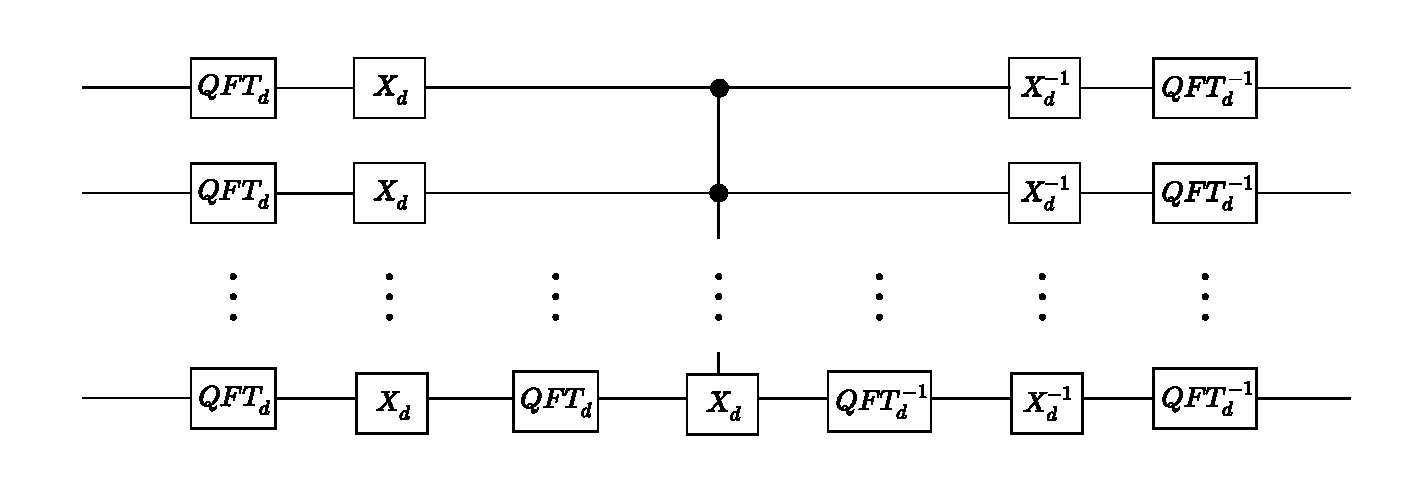
\includegraphics[scale=.45]{GGDO.pdf}

For gates see \url{https://alexheilman.com/qis/qudits}
\end{frame}

\begin{frame}{Why Qudits?/What Qudits?}

Qudits are generalization of qubits in that they're a quantum state of finite dimension $d$.\pause

$$
\vert\psi_d\rangle=\sum_{n=0}^{d-1}c_{n}\vert n \rangle
$$

Where qubits are just when $d=2$. \pause They facilitate multi-valued logic as single qu$d$it gates then allow us to encapsulate $d$th order operations.\pause As an example, the generalized $\mathbf{Z}$ gate for $d=3$

$$
\mathbf{Z_3}=\begin{bmatrix}
1 & 0 & 0\\
0 & \omega & 0 \\
0 & 0 & \omega^2\\
\end{bmatrix}
$$

\end{frame}

\begin{frame}{Generalized Grover Search (Simple Overview)}
$$
          \vert +_3 \rangle ^{\otimes 2}=
          \begin{array}{c c c c c c c c c}
          \vert 00 \rangle\\
          \vert 01 \rangle \\
          \vert 02\rangle \\ 
          \vert 10\rangle\\
          \vert 11\rangle\\
          \vert 12 \rangle \\
          \vert 20 \rangle \\
          \vert 21\rangle \\
          \vert 22 \rangle\\
          \end{array}
          \left[
          \begin{array}{c}
          1 \\
          1 \\
          1 \\
          1 \\
          1 \\
          1 \\
          1 \\
          1 \\
          1 \\
          \end{array}
          \right]\pause
          \xrightarrow{\mathcal{O}}
          \left[
          \begin{array}{c}
          1 \\
          \omega^2 \\
          \omega^2 \\
          \omega \\
          \omega^2 \\
          1 \\
          1 \\
          \omega^2 \\
          1 \\
          \end{array}
          \right]\pause
          \xrightarrow[\text{search}]{\text{Generalized Grover}}\hspace{.3cm}
          \vert 10\rangle                 
$$\pause

\begin{center}

Again we omit normalization and gritty details

\end{center}

\end{frame}

\begin{frame}{Specific Instance}

\end{frame}

\begin{frame}{Simulation}

$\bullet$ Google's Cirq allows us to simulate qudit circuits

\medskip\pause

$\bullet$ Defined generalized qutrit (i.e. $d=3$) gates

\medskip\pause

$\bullet$ Figured out several simulation techniques in Cirq

\medskip\pause 

$\bullet$ Close to functioning simulator for two qutrits (i.e. $d=3$ $n=2$)\pause , results next time \pause(hopefully)

\vspace{1cm}

The repository can be found at \url{https://github.com/tuc56407/QuditScripts}

\end{frame}

{ % all template changes are local to this group.
    \setbeamertemplate{navigation symbols}{}
    \begin{frame}{In Progress...}
        \begin{tikzpicture}[remember picture,overlay]
            \node[at=(current page.center)] {
                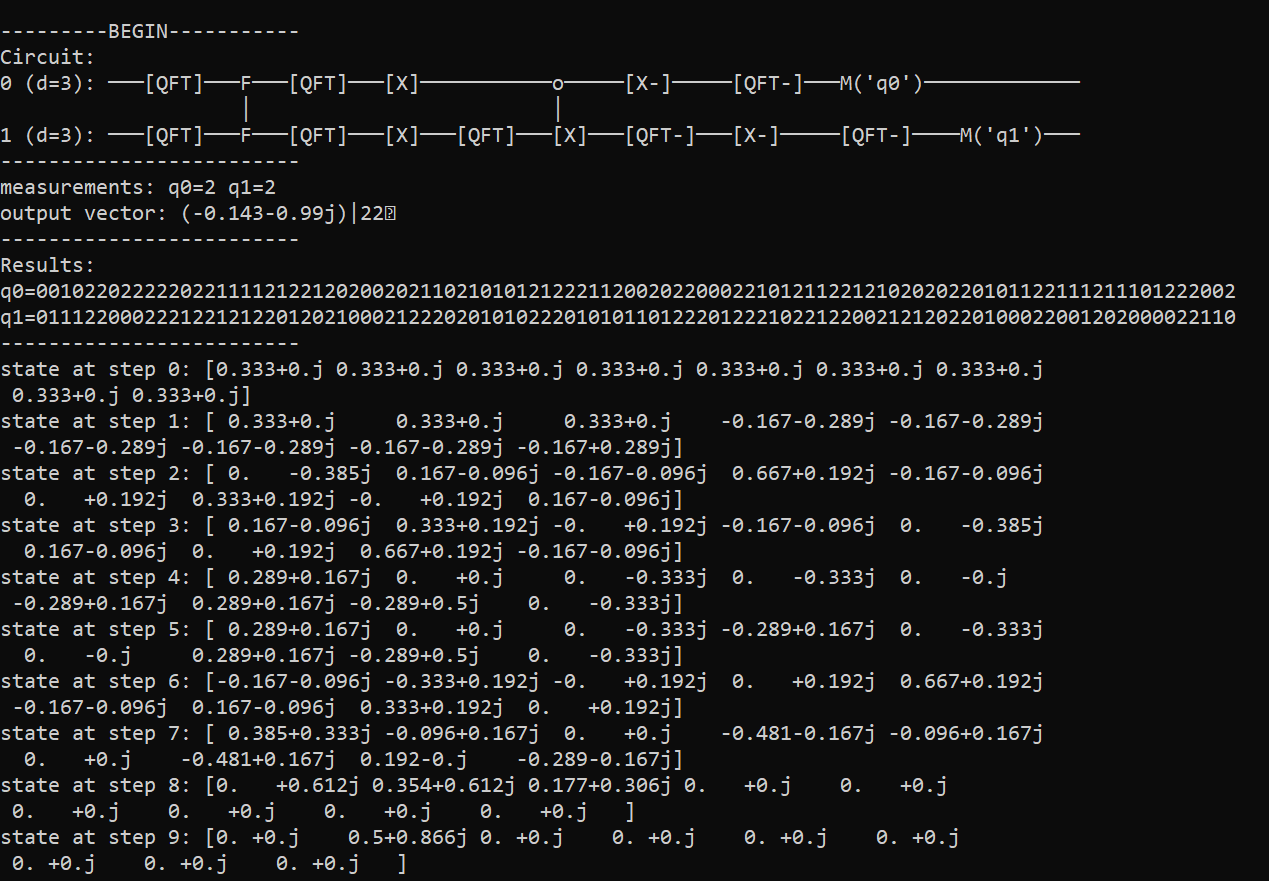
\includegraphics[keepaspectratio,
                                 width=\paperwidth,
                                 height=\paperheight]{screen.png}
            };
        \end{tikzpicture}
     \end{frame}
}

\begin{frame}{Recap}
$\bullet$ Grover search is for single binary entry in database 

\vspace{.53cm}\pause

$\bullet$ Multi-valued Grover search is recent development in field

\vspace{.53cm}\pause

$\bullet$ Progress in simulating/testing new work in Cirq


\end{frame}

\begin{frame}{What Hasn't Been Done?/Where to Go?}

$\bullet$ The recent papers only generalize strict Grover search algorithm (i.e. oracles with only one relevant solution)

\medskip\pause

$\bullet$ Natural to then generalize multi-valued amplitude amplification (Grover search for multiple solutions)

\medskip\pause

$\bullet$ With this it would be required to generalize quantum counting to the multi-valued paradigm

\medskip\pause

$\bullet$ These together would effectively give an algorithm for evaluating and counting roots of multivariate polynomial over finite fields (as they can be encoded in these types of quantum states\cite{appel2020})

\end{frame}






\begin{frame}[allowframebreaks]{References}
    % This might take more than one page
    \nocite{*}
    \printbibliography

\vspace{.5cm}

Links for work in progress


Code: \url{https://github.com/tuc56407/QuditScripts}


Overview: \url{https://alexheilman.com/qis/qudits}

\end{frame}


\end{document}
